\documentclass[13pt,oneside]{book}
\usepackage[utf8]{inputenc}
\usepackage{url}
\usepackage{listings}
\usepackage{graphicx}

\usepackage{geometry}
\geometry{a4paper, left=20mm, right=20mm, top=20mm, bottom=20mm}
\usepackage[margin=1.2in]{geometry}
\usepackage[toc,page]{appendix}
\usepackage{graphicx}
\usepackage{natbib}
\usepackage{lipsum}
\usepackage{caption}

\begin{document}

\captionsetup[figure]{margin=1.5cm,font=small,labelfont={bf},name={Figure},labelsep=colon,textfont={it}}
\captionsetup[table]{margin=1.5cm,font=small,labelfont={bf},name={Table},labelsep=colon,textfont={it}}
\setlipsumdefault{1}

\begin{titlepage}
\begin{center}
{\LARGE College Of Engineering Trivandrum}\\[3cm]
\linespread{1.2}\huge {\bfseries System Software Lab}\\[3cm]
\linespread{1}

\includegraphics[width=5cm]{img/emblem.jpeg}\\[3cm]
{\Large GOKUL K\\ S5  CSE \\ Roll No:21\\ TVE18CS021 }\\[1cm]


\textit{ }\\[2cm]
Department of Computer Science\\[0.2cm]
\today
\end{center}

\end{titlepage}

\newpage

\begin{frame}{}
    \centering
    \hspace*{-0.5cm}
    $\vcenter{\hbox{
\includegraphics[width=1.5cm]{img/emblem.jpeg}}}$
    $\vcenter{\resizebox{0.95\textwidth}{!}{
        \begin{tabular}{c}
             CS331 - System Software Lab $\cdot$ 2020 $\cdot$   \\
             \hline 
        \end{tabular}
    }}$
\end{frame}
\section*{Cycle 2}
\section*{Expt 10}
\begin{center}
    \Large{One Pass Assembler}
\end{center}
\section*{Aim}
\large
To implement a one pass assembler

\section*{Algorithm} 
    \begin{verbatim}
1 Read first line from the intermediate file .
2 Check to see if the opcode from the first line read is START . If so
then write label , opcode and operand field values of
corresponding statement directly to final output files .
3 Start the following processing for other lines in intermediate file
if it is not a comment line until an END statement is reached .
4 Start writing labels LOCCTR opcode and operand fields of
corresponding statements to the output file along with the
object code .
5 The object code is found by assembling each statement opcode
machine equivalent with the label address .
6 If there is no symbol or label in the operand field , then the
operand address is assigned as zero and it is assembled with
object code of instruction .
7 If OPCODE is BYTE , WORD , RESB etc are convert constants to object
code close operand file and exit .
	\end{verbatim}

\section*{Source Code}
\small

\begin{lstlisting}[language=C]
/* 
	Implement a single pass assembler
*/

#include <stdio.h>
#include <stdlib.h>
#include <string.h>

void itoa(int i, char *a)
{
	sprintf(a, "%d", i);
}

int main()
{
	FILE *input, *optab, *symtab, *symtab2, *output;
	char label[10], opcode[10], operand[10], name[10], optab_code[10], optab_addr[10];
	char symbol[10], symbol_addr[10], locctrs[10], ms[10], q[10], obj1[10], obj2[10];
	int start_address, locctr, prog_len, m[10], i = 0, j = 0, l = 0, k = 0;

	if(! (input = fopen("input.txt", "r")))
	{
		printf("Please make sure input.txt exists\n");
		exit(0);
	}

	if(! (optab = fopen("optab.txt", "r")))
	{
		printf("Please make sure optab.txt exists\n");
		exit(0);
	}

	symtab = fopen("symtab.txt", "w+");
	symtab2 = fopen("symtab2.txt", "w+");
	output = fopen("output.txt", "w+");

	// Checking if input file starts with a START
	fscanf(input, "%s %s %s", label, opcode, operand);
	if(strcmp(opcode, "START") == 0)
	{
		start_address = atoi(operand);
		strcpy(name, label);
		locctr = start_address;
	}

	fscanf(input, "%s %s %s", label, opcode, operand);
	while(strcmp(opcode, "END") != 0)
	{
		if(strcmp(label, "**") == 0)
		{
			while(! feof(optab))
			{
				fscanf(optab, "%s %s", optab_code, optab_addr);
				if(strcmp(optab_code, opcode) == 0)
				{
					m[i++] = locctr + 1;
					fprintf(symtab, "%s **\n", operand);
					fprintf(output, "%s 0000\n", optab_addr);
					locctr += 3;
					break;
				}
			}	
		}
		else
		{
			rewind(symtab);
			while(! feof(symtab))
			{
				fscanf(symtab, "%s %s", symbol, symbol_addr);
				if(strcmp(symbol, label) == 0)
				{
					fprintf(symtab2, "%s %d\n", label, locctr);
					fprintf(output, "%d %d\n", m[j++], locctr);
					++i;
					break;
				}
			}

			if(strcmp(opcode, "RESW") == 0)
				locctr = locctr + 3 * atoi(operand);

			else if(strcmp(opcode, "BYTE") == 0)
			{
				locctr += strlen(operand) - 2;
				for(k = 0; k < strlen(operand); ++k)
					q[l++] = operand[k];

				fprintf(output, "%s **\n", q);
				break; 
			}

			else if(strcmp(opcode, "RESB") == 0)
				locctr += atoi(operand);

			else if(strcmp(opcode, "WORD") == 0)
			{
				locctr += 3;
				fprintf(output, "%s #\n", operand);
				break;
			}
		}

		rewind(optab);
		fscanf(input, "%s %s %s", label, opcode, operand);
	}
	
	fclose(output);
	output = fopen("output.txt", "r");
	prog_len = locctr - start_address;

	printf("H^%s^%d^0%x\n", name, start_address, prog_len);
	printf("T^");
	printf("00%d^0%x", start_address, prog_len);

	while (! feof(output))
	{
		fscanf(output, "%s %s", obj1, obj2);
		if(strcmp(obj2, "0000") == 0)
			printf("^%s%s", obj1, obj2);
		
		else if(strcmp(obj2, "**") == 0)
		{
			printf("^");
			for(k = 0; k < strlen(obj1); k++)
				printf("%d", obj1[k]);
		}

		else if(strcmp(obj2, "#") == 0)
			printf("^%s", obj1);
	}

	rewind(output);
	while (! feof(output))
	{
		fscanf(output, "%s %s", obj1, obj2);
		if(
			strcmp(obj2, "0000") != 0 
			&& strcmp(obj2, "**") != 0 
			&& strcmp(obj2, "#") != 0
		)
			printf("\nT^%s^02^%s", obj1, obj2);
	}
	printf("\nE^00%d\n", start_address);
	return 0;
}
    \end{lstlisting}
    \section*{Output}
    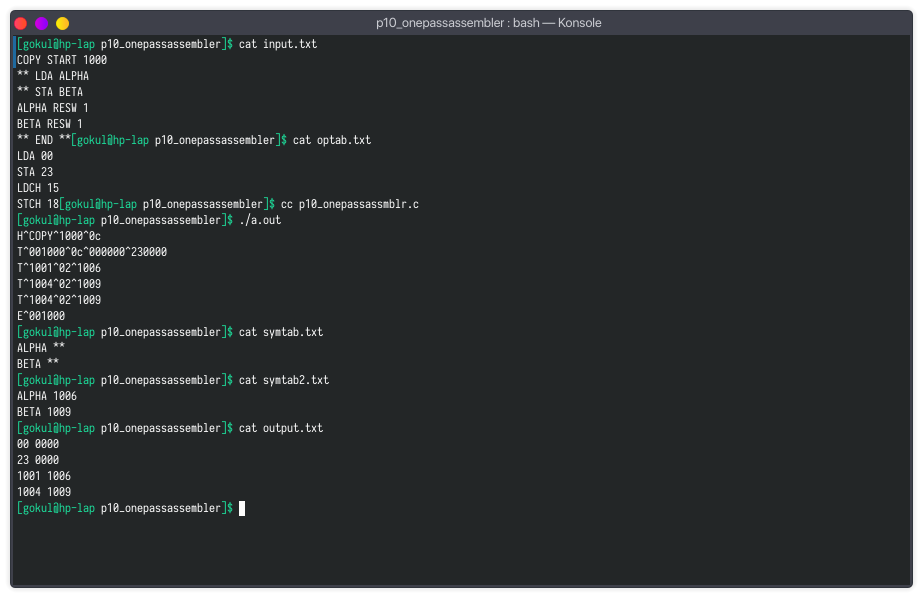
\includegraphics[width=\textwidth]{img/p10.png}
    
\Large
\section*{Result}
\large
One pass assembler is implemented and its output is verified
\end{document}